\documentclass[1p]{elsarticle_modified}
%\bibliographystyle{elsarticle-num}

%\usepackage[colorlinks]{hyperref}
%\usepackage{abbrmath_seonhwa} %\Abb, \Ascr, \Acal ,\Abf, \Afrak
\usepackage{amsfonts}
\usepackage{amssymb}
\usepackage{amsmath}
\usepackage{amsthm}
\usepackage{scalefnt}
\usepackage{amsbsy}
\usepackage{kotex}
\usepackage{caption}
\usepackage{subfig}
\usepackage{color}
\usepackage{graphicx}
\usepackage{xcolor} %% white, black, red, green, blue, cyan, magenta, yellow
\usepackage{float}
\usepackage{setspace}
\usepackage{hyperref}

\usepackage{tikz}
\usetikzlibrary{arrows}

\usepackage{multirow}
\usepackage{array} % fixed length table
\usepackage{hhline}

%%%%%%%%%%%%%%%%%%%%%
\makeatletter
\renewcommand*\env@matrix[1][\arraystretch]{%
	\edef\arraystretch{#1}%
	\hskip -\arraycolsep
	\let\@ifnextchar\new@ifnextchar
	\array{*\c@MaxMatrixCols c}}
\makeatother %https://tex.stackexchange.com/questions/14071/how-can-i-increase-the-line-spacing-in-a-matrix
%%%%%%%%%%%%%%%

\usepackage[normalem]{ulem}

\newcommand{\msout}[1]{\ifmmode\text{\sout{\ensuremath{#1}}}\else\sout{#1}\fi}
%SOURCE: \msout is \stkout macro in https://tex.stackexchange.com/questions/20609/strikeout-in-math-mode

\newcommand{\cancel}[1]{
	\ifmmode
	{\color{red}\msout{#1}}
	\else
	{\color{red}\sout{#1}}
	\fi
}

\newcommand{\add}[1]{
	{\color{blue}\uwave{#1}}
}

\newcommand{\replace}[2]{
	\ifmmode
	{\color{red}\msout{#1}}{\color{blue}\uwave{#2}}
	\else
	{\color{red}\sout{#1}}{\color{blue}\uwave{#2}}
	\fi
}

\newcommand{\Sol}{\mathcal{S}} %segment
\newcommand{\D}{D} %diagram
\newcommand{\A}{\mathcal{A}} %arc


%%%%%%%%%%%%%%%%%%%%%%%%%%%%%5 test

\def\sl{\operatorname{\textup{SL}}(2,\Cbb)}
\def\psl{\operatorname{\textup{PSL}}(2,\Cbb)}
\def\quan{\mkern 1mu \triangleright \mkern 1mu}

\theoremstyle{definition}
\newtheorem{thm}{Theorem}[section]
\newtheorem{prop}[thm]{Proposition}
\newtheorem{lem}[thm]{Lemma}
\newtheorem{ques}[thm]{Question}
\newtheorem{cor}[thm]{Corollary}
\newtheorem{defn}[thm]{Definition}
\newtheorem{exam}[thm]{Example}
\newtheorem{rmk}[thm]{Remark}
\newtheorem{alg}[thm]{Algorithm}

\newcommand{\I}{\sqrt{-1}}
\begin{document}

%\begin{frontmatter}
%
%\title{Boundary parabolic representations of knots up to 8 crossings}
%
%%% Group authors per affiliation:
%\author{Yunhi Cho} 
%\address{Department of Mathematics, University of Seoul, Seoul, Korea}
%\ead{yhcho@uos.ac.kr}
%
%
%\author{Seonhwa Kim} %\fnref{s_kim}}
%\address{Center for Geometry and Physics, Institute for Basic Science, Pohang, 37673, Korea}
%\ead{ryeona17@ibs.re.kr}
%
%\author{Hyuk Kim}
%\address{Department of Mathematical Sciences, Seoul National University, Seoul 08826, Korea}
%\ead{hyukkim@snu.ac.kr}
%
%\author{Seokbeom Yoon}
%\address{Department of Mathematical Sciences, Seoul National University, Seoul, 08826,  Korea}
%\ead{sbyoon15@snu.ac.kr}
%
%\begin{abstract}
%We find all boundary parabolic representation of knots up to 8 crossings.
%
%\end{abstract}
%\begin{keyword}
%    \MSC[2010] 57M25 
%\end{keyword}
%
%\end{frontmatter}

%\linenumbers
%\tableofcontents
%
\newcommand\colored[1]{\textcolor{white}{\rule[-0.35ex]{0.8em}{1.4ex}}\kern-0.8em\color{red} #1}%
%\newcommand\colored[1]{\textcolor{white}{ #1}\kern-2.17ex	\textcolor{white}{ #1}\kern-1.81ex	\textcolor{white}{ #1}\kern-2.15ex\color{red}#1	}

{\Large $\underline{12n_{0289}~(K12n_{0289})}$}

\setlength{\tabcolsep}{10pt}
\renewcommand{\arraystretch}{1.6}
\vspace{1cm}\begin{tabular}{m{100pt}>{\centering\arraybackslash}m{274pt}}
\multirow{5}{120pt}{
	\centering
	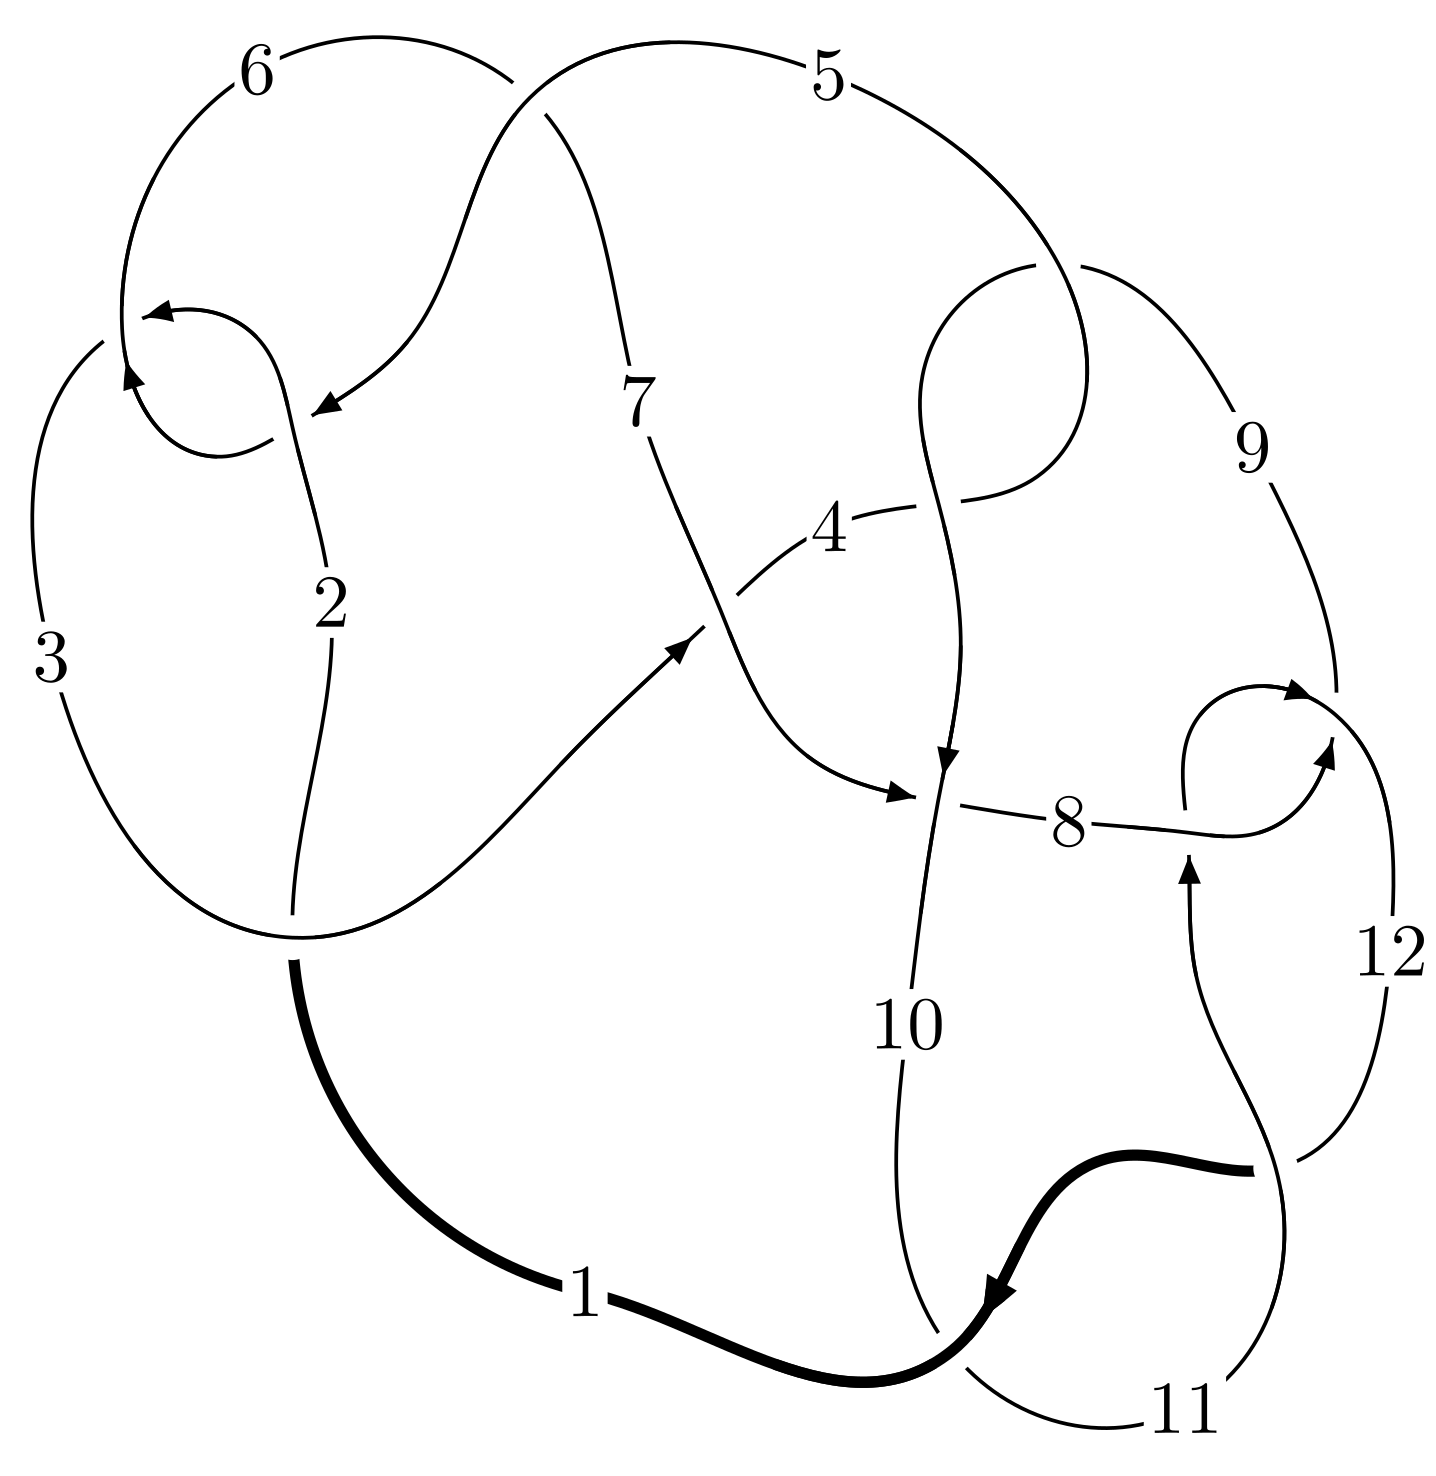
\includegraphics[width=112pt]{../../../GIT/diagram.site/Diagrams/png/2378_12n_0289.png}\\
\ \ \ A knot diagram\footnotemark}&
\allowdisplaybreaks
\textbf{Linearized knot diagam} \\
\cline{2-2}
 &
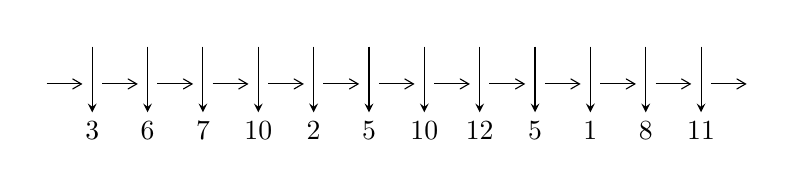
\begin{tikzpicture}[x=20pt, y=17pt]
	% nodes
	\node (C0) at (0, 0) {};
	\node (C1) at (1, 0) {};
	\node (C1U) at (1, +1) {};
	\node (C1D) at (1, -1) {3};

	\node (C2) at (2, 0) {};
	\node (C2U) at (2, +1) {};
	\node (C2D) at (2, -1) {6};

	\node (C3) at (3, 0) {};
	\node (C3U) at (3, +1) {};
	\node (C3D) at (3, -1) {7};

	\node (C4) at (4, 0) {};
	\node (C4U) at (4, +1) {};
	\node (C4D) at (4, -1) {10};

	\node (C5) at (5, 0) {};
	\node (C5U) at (5, +1) {};
	\node (C5D) at (5, -1) {2};

	\node (C6) at (6, 0) {};
	\node (C6U) at (6, +1) {};
	\node (C6D) at (6, -1) {5};

	\node (C7) at (7, 0) {};
	\node (C7U) at (7, +1) {};
	\node (C7D) at (7, -1) {10};

	\node (C8) at (8, 0) {};
	\node (C8U) at (8, +1) {};
	\node (C8D) at (8, -1) {12};

	\node (C9) at (9, 0) {};
	\node (C9U) at (9, +1) {};
	\node (C9D) at (9, -1) {5};

	\node (C10) at (10, 0) {};
	\node (C10U) at (10, +1) {};
	\node (C10D) at (10, -1) {1};

	\node (C11) at (11, 0) {};
	\node (C11U) at (11, +1) {};
	\node (C11D) at (11, -1) {8};

	\node (C12) at (12, 0) {};
	\node (C12U) at (12, +1) {};
	\node (C12D) at (12, -1) {11};
	\node (C13) at (13, 0) {};

	% arrows
	\draw[->,>={angle 60}]
	(C0) edge (C1) (C1) edge (C2) (C2) edge (C3) (C3) edge (C4) (C4) edge (C5) (C5) edge (C6) (C6) edge (C7) (C7) edge (C8) (C8) edge (C9) (C9) edge (C10) (C10) edge (C11) (C11) edge (C12) (C12) edge (C13) ;	\draw[->,>=stealth]
	(C1U) edge (C1D) (C2U) edge (C2D) (C3U) edge (C3D) (C4U) edge (C4D) (C5U) edge (C5D) (C6U) edge (C6D) (C7U) edge (C7D) (C8U) edge (C8D) (C9U) edge (C9D) (C10U) edge (C10D) (C11U) edge (C11D) (C12U) edge (C12D) ;
	\end{tikzpicture} \\
\hhline{~~} \\& 
\textbf{Solving Sequence} \\ \cline{2-2} 
 &
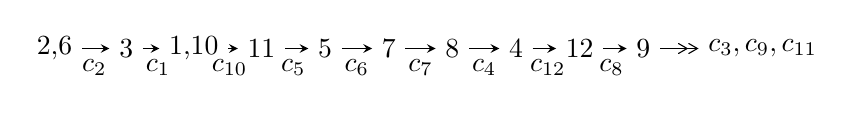
\begin{tikzpicture}[x=23pt, y=7pt]
	% node
	\node (A0) at (-1/8, 0) {2,6};
	\node (A1) at (1, 0) {3};
	\node (A2) at (33/16, 0) {1,10};
	\node (A3) at (25/8, 0) {11};
	\node (A4) at (33/8, 0) {5};
	\node (A5) at (41/8, 0) {7};
	\node (A6) at (49/8, 0) {8};
	\node (A7) at (57/8, 0) {4};
	\node (A8) at (65/8, 0) {12};
	\node (A9) at (73/8, 0) {9};
	\node (C1) at (1/2, -1) {$c_{2}$};
	\node (C2) at (3/2, -1) {$c_{1}$};
	\node (C3) at (21/8, -1) {$c_{10}$};
	\node (C4) at (29/8, -1) {$c_{5}$};
	\node (C5) at (37/8, -1) {$c_{6}$};
	\node (C6) at (45/8, -1) {$c_{7}$};
	\node (C7) at (53/8, -1) {$c_{4}$};
	\node (C8) at (61/8, -1) {$c_{12}$};
	\node (C9) at (69/8, -1) {$c_{8}$};
	\node (A10) at (11, 0) {$c_{3},c_{9},c_{11}$};

	% edge
	\draw[->,>=stealth]	
	(A0) edge (A1) (A1) edge (A2) (A2) edge (A3) (A3) edge (A4) (A4) edge (A5) (A5) edge (A6) (A6) edge (A7) (A7) edge (A8) (A8) edge (A9) ;
	\draw[->>,>={angle 60}]	
	(A9) edge (A10);
\end{tikzpicture} \\ 

\end{tabular} \\

\footnotetext{
The image of knot diagram is generated by the software ``\textbf{Draw programme}" developed by Andrew Bartholomew(\url{http://www.layer8.co.uk/maths/draw/index.htm\#Running-draw}), where we modified some parts for our purpose(\url{https://github.com/CATsTAILs/LinksPainter}).
}\phantom \\ \newline 
\centering \textbf{Ideals for irreducible components\footnotemark of $X_{\text{par}}$} 
 
\begin{align*}
I^u_{1}&=\langle 
u^8-2 u^6+u^5+2 u^4- u^3- u^2+b+u,\;- u^{11}+2 u^9-4 u^7+4 u^5-2 u^4-3 u^3+2 u^2+a+2 u-2,\\
\phantom{I^u_{1}}&\phantom{= \langle  }u^{12}- u^{11}-2 u^{10}+3 u^9+3 u^8-5 u^7-2 u^6+6 u^5-4 u^3+3 u-1\rangle \\
I^u_{2}&=\langle 
-3 u^{41}+7 u^{40}+\cdots+2 b+7,\;3 u^{41}-5 u^{40}+\cdots+2 a+5,\;u^{42}-3 u^{41}+\cdots-2 u+1\rangle \\
I^u_{3}&=\langle 
b+u,\;a+u,\;u^3+u^2-1\rangle \\
I^u_{4}&=\langle 
b- a,\;u^2 a+a^2+u^2+2 u+1,\;u^3+u^2-1\rangle \\
\\
\end{align*}
\raggedright * 4 irreducible components of $\dim_{\mathbb{C}}=0$, with total 63 representations.\\
\footnotetext{All coefficients of polynomials are rational numbers. But the coefficients are sometimes approximated in decimal forms when there is not enough margin.}
\newpage
\renewcommand{\arraystretch}{1}
\centering \section*{I. $I^u_{1}= \langle u^8-2 u^6+u^5+2 u^4- u^3- u^2+b+u,\;- u^{11}+2 u^9+\cdots+a-2,\;u^{12}- u^{11}+\cdots+3 u-1 \rangle$}
\flushleft \textbf{(i) Arc colorings}\\
\begin{tabular}{m{7pt} m{180pt} m{7pt} m{180pt} }
\flushright $a_{2}=$&$\begin{pmatrix}1\\0\end{pmatrix}$ \\
\flushright $a_{6}=$&$\begin{pmatrix}0\\u\end{pmatrix}$ \\
\flushright $a_{3}=$&$\begin{pmatrix}1\\u^2\end{pmatrix}$ \\
\flushright $a_{1}=$&$\begin{pmatrix}- u^2+1\\- u^4\end{pmatrix}$ \\
\flushright $a_{10}=$&$\begin{pmatrix}u^{11}-2 u^9+4 u^7-4 u^5+2 u^4+3 u^3-2 u^2-2 u+2\\- u^8+2 u^6- u^5-2 u^4+u^3+u^2- u\end{pmatrix}$ \\
\flushright $a_{11}=$&$\begin{pmatrix}u^{11}-2 u^9+4 u^7-4 u^5+u^4+3 u^3- u^2-2 u+2\\- u^8+u^6- u^5-2 u^4+u^3+u^2- u\end{pmatrix}$ \\
\flushright $a_{5}=$&$\begin{pmatrix}u\\u\end{pmatrix}$ \\
\flushright $a_{7}=$&$\begin{pmatrix}- u^3\\- u^3+u\end{pmatrix}$ \\
\flushright $a_{8}=$&$\begin{pmatrix}- u^9+2 u^7- u^6-3 u^5+u^4+2 u^3- u^2- u\\- u^9+2 u^7- u^6-3 u^5+2 u^4+2 u^3-2 u^2- u+1\end{pmatrix}$ \\
\flushright $a_{4}=$&$\begin{pmatrix}- u^8+u^6- u^4+1\\- u^8+2 u^6-2 u^4+2 u^2\end{pmatrix}$ \\
\flushright $a_{12}=$&$\begin{pmatrix}u^{11}- u^{10}-2 u^9+2 u^8+3 u^7-3 u^6-3 u^5+3 u^4+2 u^3-2 u^2-2 u+2\\- u^{10}+u^8- u^7-2 u^6+u^5- u^3\end{pmatrix}$ \\
\flushright $a_{9}=$&$\begin{pmatrix}- u^4+u^2-1\\u^{11}-2 u^9+u^8+4 u^7-2 u^6-3 u^5+3 u^4+2 u^3-2 u^2- u+1\end{pmatrix}$\\&\end{tabular}
\flushleft \textbf{(ii) Obstruction class $= -1$}\\~\\
\flushleft \textbf{(iii) Cusp Shapes $= 4 u^{11}-6 u^9+12 u^7+2 u^6-8 u^5+2 u^4+8 u^3+2 u^2-8 u-10$}\\~\\
\newpage\renewcommand{\arraystretch}{1}
\flushleft \textbf{(iv) u-Polynomials at the component}\newline \\
\begin{tabular}{m{50pt}|m{274pt}}
Crossings & \hspace{64pt}u-Polynomials at each crossing \\
\hline $$\begin{aligned}c_{1},c_{6},c_{10}\\c_{12}\end{aligned}$$&$\begin{aligned}
&u^{12}+5 u^{11}+\cdots+9 u+1
\end{aligned}$\\
\hline $$\begin{aligned}c_{2},c_{5},c_{8}\\c_{11}\end{aligned}$$&$\begin{aligned}
&u^{12}+u^{11}-2 u^{10}-3 u^9+3 u^8+5 u^7-2 u^6-6 u^5+4 u^3-3 u-1
\end{aligned}$\\
\hline $$\begin{aligned}c_{3},c_{7}\end{aligned}$$&$\begin{aligned}
&u^{12}- u^{11}+\cdots-5 u-1
\end{aligned}$\\
\hline $$\begin{aligned}c_{4},c_{9}\end{aligned}$$&$\begin{aligned}
&u^{12}+7 u^{11}+\cdots+32 u+8
\end{aligned}$\\
\hline
\end{tabular}\\~\\
\newpage\renewcommand{\arraystretch}{1}
\flushleft \textbf{(v) Riley Polynomials at the component}\newline \\
\begin{tabular}{m{50pt}|m{274pt}}
Crossings & \hspace{64pt}Riley Polynomials at each crossing \\
\hline $$\begin{aligned}c_{1},c_{6},c_{10}\\c_{12}\end{aligned}$$&$\begin{aligned}
&y^{12}+7 y^{11}+\cdots-33 y+1
\end{aligned}$\\
\hline $$\begin{aligned}c_{2},c_{5},c_{8}\\c_{11}\end{aligned}$$&$\begin{aligned}
&y^{12}-5 y^{11}+\cdots-9 y+1
\end{aligned}$\\
\hline $$\begin{aligned}c_{3},c_{7}\end{aligned}$$&$\begin{aligned}
&y^{12}-17 y^{11}+\cdots-9 y+1
\end{aligned}$\\
\hline $$\begin{aligned}c_{4},c_{9}\end{aligned}$$&$\begin{aligned}
&y^{12}-7 y^{11}+\cdots-192 y+64
\end{aligned}$\\
\hline
\end{tabular}\\~\\
\newpage\flushleft \textbf{(vi) Complex Volumes and Cusp Shapes}
$$\begin{array}{c|c|c}  
\text{Solutions to }I^u_{1}& \I (\text{vol} + \sqrt{-1}CS) & \text{Cusp shape}\\
 \hline 
\begin{aligned}
u &= \phantom{-}0.921925 + 0.343588 I \\
a &= -0.611717 + 0.476706 I \\
b &= \phantom{-}0.056760 - 0.351806 I\end{aligned}
 & -2.36994 - 2.76031 I & -17.1687 + 5.8086 I \\ \hline\begin{aligned}
u &= \phantom{-}0.921925 - 0.343588 I \\
a &= -0.611717 - 0.476706 I \\
b &= \phantom{-}0.056760 + 0.351806 I\end{aligned}
 & -2.36994 + 2.76031 I & -17.1687 - 5.8086 I \\ \hline\begin{aligned}
u &= \phantom{-}0.588705 + 0.829892 I \\
a &= \phantom{-}1.69413 - 0.79218 I \\
b &= \phantom{-}1.295740 + 0.564858 I\end{aligned}
 & -0.17368 + 3.06646 I & -8.92631 - 0.43083 I \\ \hline\begin{aligned}
u &= \phantom{-}0.588705 - 0.829892 I \\
a &= \phantom{-}1.69413 + 0.79218 I \\
b &= \phantom{-}1.295740 - 0.564858 I\end{aligned}
 & -0.17368 - 3.06646 I & -8.92631 + 0.43083 I \\ \hline\begin{aligned}
u &= -0.700347 + 0.661080 I \\
a &= \phantom{-}0.49057 + 1.67492 I \\
b &= \phantom{-}1.37850 + 1.19320 I\end{aligned}
 & \phantom{-}3.36282 + 2.18981 I & -7.17700 - 3.81343 I \\ \hline\begin{aligned}
u &= -0.700347 - 0.661080 I \\
a &= \phantom{-}0.49057 - 1.67492 I \\
b &= \phantom{-}1.37850 - 1.19320 I\end{aligned}
 & \phantom{-}3.36282 - 2.18981 I & -7.17700 + 3.81343 I \\ \hline\begin{aligned}
u &= -0.993915 + 0.611197 I \\
a &= -1.53521 - 1.43733 I \\
b &= -2.02283 - 0.51409 I\end{aligned}
 & \phantom{-}1.49384 + 7.77925 I & -11.7273 - 7.9652 I \\ \hline\begin{aligned}
u &= -0.993915 - 0.611197 I \\
a &= -1.53521 + 1.43733 I \\
b &= -2.02283 + 0.51409 I\end{aligned}
 & \phantom{-}1.49384 - 7.77925 I & -11.7273 + 7.9652 I \\ \hline\begin{aligned}
u &= -1.18481\phantom{ +0.000000I} \\
a &= -0.513967\phantom{ +0.000000I} \\
b &= \phantom{-}0.968302\phantom{ +0.000000I}\end{aligned}
 & -12.5188\phantom{ +0.000000I} & -20.4260\phantom{ +0.000000I} \\ \hline\begin{aligned}
u &= \phantom{-}1.073430 + 0.702670 I \\
a &= -0.31962 + 2.22050 I \\
b &= -1.57673 + 2.45459 I\end{aligned}
 & -3.0728 - 14.5878 I & -12.5949 + 9.1386 I\\
 \hline 
 \end{array}$$\newpage$$\begin{array}{c|c|c}  
\text{Solutions to }I^u_{1}& \I (\text{vol} + \sqrt{-1}CS) & \text{Cusp shape}\\
 \hline 
\begin{aligned}
u &= \phantom{-}1.073430 - 0.702670 I \\
a &= -0.31962 - 2.22050 I \\
b &= -1.57673 - 2.45459 I\end{aligned}
 & -3.0728 + 14.5878 I & -12.5949 - 9.1386 I \\ \hline\begin{aligned}
u &= \phantom{-}0.405199\phantom{ +0.000000I} \\
a &= \phantom{-}1.07767\phantom{ +0.000000I} \\
b &= -0.231197\phantom{ +0.000000I}\end{aligned}
 & -0.765991\phantom{ +0.000000I} & -12.3860\phantom{ +0.000000I}\\
 \hline 
 \end{array}$$\newpage\newpage\renewcommand{\arraystretch}{1}
\centering \section*{II. $I^u_{2}= \langle -3 u^{41}+7 u^{40}+\cdots+2 b+7,\;3 u^{41}-5 u^{40}+\cdots+2 a+5,\;u^{42}-3 u^{41}+\cdots-2 u+1 \rangle$}
\flushleft \textbf{(i) Arc colorings}\\
\begin{tabular}{m{7pt} m{180pt} m{7pt} m{180pt} }
\flushright $a_{2}=$&$\begin{pmatrix}1\\0\end{pmatrix}$ \\
\flushright $a_{6}=$&$\begin{pmatrix}0\\u\end{pmatrix}$ \\
\flushright $a_{3}=$&$\begin{pmatrix}1\\u^2\end{pmatrix}$ \\
\flushright $a_{1}=$&$\begin{pmatrix}- u^2+1\\- u^4\end{pmatrix}$ \\
\flushright $a_{10}=$&$\begin{pmatrix}-\frac{3}{2} u^{41}+\frac{5}{2} u^{40}+\cdots+\frac{21}{2} u-\frac{5}{2}\\\frac{3}{2} u^{41}-\frac{7}{2} u^{40}+\cdots+\frac{15}{2} u-\frac{7}{2}\end{pmatrix}$ \\
\flushright $a_{11}=$&$\begin{pmatrix}\frac{11}{2} u^{41}-15 u^{40}+\cdots+17 u-\frac{17}{2}\\7 u^{41}-\frac{35}{2} u^{40}+\cdots+\frac{31}{2} u-\frac{21}{2}\end{pmatrix}$ \\
\flushright $a_{5}=$&$\begin{pmatrix}u\\u\end{pmatrix}$ \\
\flushright $a_{7}=$&$\begin{pmatrix}- u^3\\- u^3+u\end{pmatrix}$ \\
\flushright $a_{8}=$&$\begin{pmatrix}\frac{1}{2} u^{39}- u^{38}+\cdots+u-\frac{1}{2}\\\frac{1}{2} u^{39}- u^{38}+\cdots+u+\frac{1}{2}\end{pmatrix}$ \\
\flushright $a_{4}=$&$\begin{pmatrix}- u^8+u^6- u^4+1\\- u^8+2 u^6-2 u^4+2 u^2\end{pmatrix}$ \\
\flushright $a_{12}=$&$\begin{pmatrix}\frac{1}{2} u^{41}-\frac{3}{2} u^{40}+\cdots-\frac{1}{2} u+1\\-\frac{1}{2} u^{40}+\frac{9}{2} u^{38}+\cdots+\frac{1}{2} u-1\end{pmatrix}$ \\
\flushright $a_{9}=$&$\begin{pmatrix}-\frac{3}{2} u^{41}+\frac{9}{2} u^{40}+\cdots-\frac{27}{2} u+\frac{11}{2}\\-\frac{9}{2} u^{41}+\frac{21}{2} u^{40}+\cdots-\frac{21}{2} u+\frac{13}{2}\end{pmatrix}$\\&\end{tabular}
\flushleft \textbf{(ii) Obstruction class $= -1$}\\~\\
\flushleft \textbf{(iii) Cusp Shapes $= - u^{41}-\frac{9}{2} u^{40}+\cdots-\frac{45}{2} u-\frac{21}{2}$}\\~\\
\newpage\renewcommand{\arraystretch}{1}
\flushleft \textbf{(iv) u-Polynomials at the component}\newline \\
\begin{tabular}{m{50pt}|m{274pt}}
Crossings & \hspace{64pt}u-Polynomials at each crossing \\
\hline $$\begin{aligned}c_{1},c_{6},c_{10}\\c_{12}\end{aligned}$$&$\begin{aligned}
&u^{42}+15 u^{41}+\cdots+20 u+1
\end{aligned}$\\
\hline $$\begin{aligned}c_{2},c_{5},c_{8}\\c_{11}\end{aligned}$$&$\begin{aligned}
&u^{42}+3 u^{41}+\cdots+2 u+1
\end{aligned}$\\
\hline $$\begin{aligned}c_{3},c_{7}\end{aligned}$$&$\begin{aligned}
&u^{42}-3 u^{41}+\cdots+24 u+1
\end{aligned}$\\
\hline $$\begin{aligned}c_{4},c_{9}\end{aligned}$$&$\begin{aligned}
&(u^{21}-3 u^{20}+\cdots-4 u+8)^{2}
\end{aligned}$\\
\hline
\end{tabular}\\~\\
\newpage\renewcommand{\arraystretch}{1}
\flushleft \textbf{(v) Riley Polynomials at the component}\newline \\
\begin{tabular}{m{50pt}|m{274pt}}
Crossings & \hspace{64pt}Riley Polynomials at each crossing \\
\hline $$\begin{aligned}c_{1},c_{6},c_{10}\\c_{12}\end{aligned}$$&$\begin{aligned}
&y^{42}+25 y^{41}+\cdots-12 y+1
\end{aligned}$\\
\hline $$\begin{aligned}c_{2},c_{5},c_{8}\\c_{11}\end{aligned}$$&$\begin{aligned}
&y^{42}-15 y^{41}+\cdots-20 y+1
\end{aligned}$\\
\hline $$\begin{aligned}c_{3},c_{7}\end{aligned}$$&$\begin{aligned}
&y^{42}-35 y^{41}+\cdots-372 y+1
\end{aligned}$\\
\hline $$\begin{aligned}c_{4},c_{9}\end{aligned}$$&$\begin{aligned}
&(y^{21}-21 y^{20}+\cdots+80 y-64)^{2}
\end{aligned}$\\
\hline
\end{tabular}\\~\\
\newpage\flushleft \textbf{(vi) Complex Volumes and Cusp Shapes}
$$\begin{array}{c|c|c}  
\text{Solutions to }I^u_{2}& \I (\text{vol} + \sqrt{-1}CS) & \text{Cusp shape}\\
 \hline 
\begin{aligned}
u &= \phantom{-}1.001590 + 0.071446 I \\
a &= -0.247034 + 0.982841 I \\
b &= -0.0703049 - 0.0213694 I\end{aligned}
 & -1.68246 + 2.02701 I & -16.1395 - 3.2075 I \\ \hline\begin{aligned}
u &= \phantom{-}1.001590 - 0.071446 I \\
a &= -0.247034 - 0.982841 I \\
b &= -0.0703049 + 0.0213694 I\end{aligned}
 & -1.68246 - 2.02701 I & -16.1395 + 3.2075 I \\ \hline\begin{aligned}
u &= -0.884746 + 0.507709 I \\
a &= -1.00430 - 1.65860 I \\
b &= -1.70041 - 0.93550 I\end{aligned}
 & -1.68246 + 2.02701 I & -16.1395 - 3.2075 I \\ \hline\begin{aligned}
u &= -0.884746 - 0.507709 I \\
a &= -1.00430 + 1.65860 I \\
b &= -1.70041 + 0.93550 I\end{aligned}
 & -1.68246 - 2.02701 I & -16.1395 + 3.2075 I \\ \hline\begin{aligned}
u &= \phantom{-}0.498112 + 0.843586 I \\
a &= -1.51048 + 0.33957 I \\
b &= -0.92205 - 1.13548 I\end{aligned}
 & -6.44569 + 1.90498 I & -15.1767 - 0.6933 I \\ \hline\begin{aligned}
u &= \phantom{-}0.498112 - 0.843586 I \\
a &= -1.51048 - 0.33957 I \\
b &= -0.92205 + 1.13548 I\end{aligned}
 & -6.44569 - 1.90498 I & -15.1767 + 0.6933 I \\ \hline\begin{aligned}
u &= \phantom{-}0.833041 + 0.624453 I \\
a &= -0.244467 - 1.048030 I \\
b &= -0.795422 - 0.433395 I\end{aligned}
 & \phantom{-}4.76367 + 0.56948 I & -11.53430 - 0.71170 I \\ \hline\begin{aligned}
u &= \phantom{-}0.833041 - 0.624453 I \\
a &= -0.244467 + 1.048030 I \\
b &= -0.795422 + 0.433395 I\end{aligned}
 & \phantom{-}4.76367 - 0.56948 I & -11.53430 + 0.71170 I \\ \hline\begin{aligned}
u &= \phantom{-}0.589823 + 0.864603 I \\
a &= -1.89138 + 0.71030 I \\
b &= -1.53680 - 0.72844 I\end{aligned}
 & -1.59942 + 8.75882 I & -10.82911 - 4.89320 I \\ \hline\begin{aligned}
u &= \phantom{-}0.589823 - 0.864603 I \\
a &= -1.89138 - 0.71030 I \\
b &= -1.53680 + 0.72844 I\end{aligned}
 & -1.59942 - 8.75882 I & -10.82911 + 4.89320 I\\
 \hline 
 \end{array}$$\newpage$$\begin{array}{c|c|c}  
\text{Solutions to }I^u_{2}& \I (\text{vol} + \sqrt{-1}CS) & \text{Cusp shape}\\
 \hline 
\begin{aligned}
u &= \phantom{-}0.865106 + 0.622456 I \\
a &= \phantom{-}0.478460 + 0.785204 I \\
b &= \phantom{-}1.077610 + 0.227526 I\end{aligned}
 & \phantom{-}4.66319 - 5.46111 I & -12.12408 + 5.29794 I \\ \hline\begin{aligned}
u &= \phantom{-}0.865106 - 0.622456 I \\
a &= \phantom{-}0.478460 - 0.785204 I \\
b &= \phantom{-}1.077610 - 0.227526 I\end{aligned}
 & \phantom{-}4.66319 + 5.46111 I & -12.12408 - 5.29794 I \\ \hline\begin{aligned}
u &= \phantom{-}0.370195 + 0.797477 I \\
a &= -0.975137 + 0.163149 I \\
b &= -0.109542 - 1.285730 I\end{aligned}
 & -2.89368 - 5.09092 I & -11.85705 + 4.85512 I \\ \hline\begin{aligned}
u &= \phantom{-}0.370195 - 0.797477 I \\
a &= -0.975137 - 0.163149 I \\
b &= -0.109542 + 1.285730 I\end{aligned}
 & -2.89368 + 5.09092 I & -11.85705 - 4.85512 I \\ \hline\begin{aligned}
u &= -0.877054 + 0.709305 I \\
a &= \phantom{-}0.621738 + 0.723259 I \\
b &= \phantom{-}0.924556 + 0.344996 I\end{aligned}
 & \phantom{-}2.39962 + 2.72155 I & -2.38517 - 1.80674 I \\ \hline\begin{aligned}
u &= -0.877054 - 0.709305 I \\
a &= \phantom{-}0.621738 - 0.723259 I \\
b &= \phantom{-}0.924556 - 0.344996 I\end{aligned}
 & \phantom{-}2.39962 - 2.72155 I & -2.38517 + 1.80674 I \\ \hline\begin{aligned}
u &= -1.140080 + 0.053957 I \\
a &= \phantom{-}0.121069 - 0.443029 I \\
b &= -1.234320 - 0.298114 I\end{aligned}
 & -6.44569 + 1.90498 I & -15.1767 - 0.6933 I \\ \hline\begin{aligned}
u &= -1.140080 - 0.053957 I \\
a &= \phantom{-}0.121069 + 0.443029 I \\
b &= -1.234320 + 0.298114 I\end{aligned}
 & -6.44569 - 1.90498 I & -15.1767 + 0.6933 I \\ \hline\begin{aligned}
u &= -0.948500 + 0.657394 I \\
a &= \phantom{-}1.35145 + 1.05024 I \\
b &= \phantom{-}1.70425 + 0.27722 I\end{aligned}
 & \phantom{-}2.62978 + 2.94639 I & -8.38979 - 1.94831 I \\ \hline\begin{aligned}
u &= -0.948500 - 0.657394 I \\
a &= \phantom{-}1.35145 - 1.05024 I \\
b &= \phantom{-}1.70425 - 0.27722 I\end{aligned}
 & \phantom{-}2.62978 - 2.94639 I & -8.38979 + 1.94831 I\\
 \hline 
 \end{array}$$\newpage$$\begin{array}{c|c|c}  
\text{Solutions to }I^u_{2}& \I (\text{vol} + \sqrt{-1}CS) & \text{Cusp shape}\\
 \hline 
\begin{aligned}
u &= \phantom{-}0.440380 + 0.720566 I \\
a &= \phantom{-}1.022170 - 0.478261 I \\
b &= \phantom{-}0.238333 + 0.804288 I\end{aligned}
 & -1.18994\phantom{ +0.000000I} & -9.46820 + 0. I\phantom{ +0.000000I} \\ \hline\begin{aligned}
u &= \phantom{-}0.440380 - 0.720566 I \\
a &= \phantom{-}1.022170 + 0.478261 I \\
b &= \phantom{-}0.238333 - 0.804288 I\end{aligned}
 & -1.18994\phantom{ +0.000000I} & -9.46820 + 0. I\phantom{ +0.000000I} \\ \hline\begin{aligned}
u &= -0.602886 + 0.586036 I \\
a &= -0.56399 - 1.78814 I \\
b &= -1.51211 - 1.10890 I\end{aligned}
 & \phantom{-}2.62978 - 2.94639 I & -8.38979 + 1.94831 I \\ \hline\begin{aligned}
u &= -0.602886 - 0.586036 I \\
a &= -0.56399 + 1.78814 I \\
b &= -1.51211 + 1.10890 I\end{aligned}
 & \phantom{-}2.62978 + 2.94639 I & -8.38979 - 1.94831 I \\ \hline\begin{aligned}
u &= -1.169360 + 0.079358 I \\
a &= -0.342452 + 0.671662 I \\
b &= \phantom{-}1.087440 + 0.452577 I\end{aligned}
 & -8.23029 + 7.48200 I & -17.0704 - 5.2473 I \\ \hline\begin{aligned}
u &= -1.169360 - 0.079358 I \\
a &= -0.342452 - 0.671662 I \\
b &= \phantom{-}1.087440 - 0.452577 I\end{aligned}
 & -8.23029 - 7.48200 I & -17.0704 + 5.2473 I \\ \hline\begin{aligned}
u &= -0.869430 + 0.810182 I \\
a &= -0.90284 + 1.14540 I \\
b &= -0.28767 + 1.52547 I\end{aligned}
 & \phantom{-}4.76367 + 0.56948 I & -11.53430 - 0.71170 I \\ \hline\begin{aligned}
u &= -0.869430 - 0.810182 I \\
a &= -0.90284 - 1.14540 I \\
b &= -0.28767 - 1.52547 I\end{aligned}
 & \phantom{-}4.76367 - 0.56948 I & -11.53430 + 0.71170 I \\ \hline\begin{aligned}
u &= -0.903021 + 0.803753 I \\
a &= \phantom{-}1.23931 - 0.82374 I \\
b &= \phantom{-}0.76478 - 1.36737 I\end{aligned}
 & \phantom{-}4.66319 + 5.46111 I & -12.00000 - 5.29794 I \\ \hline\begin{aligned}
u &= -0.903021 - 0.803753 I \\
a &= \phantom{-}1.23931 + 0.82374 I \\
b &= \phantom{-}0.76478 + 1.36737 I\end{aligned}
 & \phantom{-}4.66319 - 5.46111 I & -12.00000 + 5.29794 I\\
 \hline 
 \end{array}$$\newpage$$\begin{array}{c|c|c}  
\text{Solutions to }I^u_{2}& \I (\text{vol} + \sqrt{-1}CS) & \text{Cusp shape}\\
 \hline 
\begin{aligned}
u &= \phantom{-}1.054680 + 0.618331 I \\
a &= -0.151148 - 1.199150 I \\
b &= \phantom{-}0.95395 - 1.70109 I\end{aligned}
 & -2.89368 - 5.09092 I & -12.00000 + 4.85512 I \\ \hline\begin{aligned}
u &= \phantom{-}1.054680 - 0.618331 I \\
a &= -0.151148 + 1.199150 I \\
b &= \phantom{-}0.95395 + 1.70109 I\end{aligned}
 & -2.89368 + 5.09092 I & -12.00000 - 4.85512 I \\ \hline\begin{aligned}
u &= \phantom{-}1.086360 + 0.586494 I \\
a &= \phantom{-}0.636112 + 1.121460 I \\
b &= -0.52511 + 1.74837 I\end{aligned}
 & -5.00675\phantom{ +0.000000I} & -15.0273 + 0. I\phantom{ +0.000000I} \\ \hline\begin{aligned}
u &= \phantom{-}1.086360 - 0.586494 I \\
a &= \phantom{-}0.636112 - 1.121460 I \\
b &= -0.52511 - 1.74837 I\end{aligned}
 & -5.00675\phantom{ +0.000000I} & -15.0273 + 0. I\phantom{ +0.000000I} \\ \hline\begin{aligned}
u &= \phantom{-}1.060980 + 0.690081 I \\
a &= \phantom{-}0.35900 - 1.97361 I \\
b &= \phantom{-}1.55493 - 2.24059 I\end{aligned}
 & -1.59942 - 8.75882 I & -10.82911 + 4.89320 I \\ \hline\begin{aligned}
u &= \phantom{-}1.060980 - 0.690081 I \\
a &= \phantom{-}0.35900 + 1.97361 I \\
b &= \phantom{-}1.55493 + 2.24059 I\end{aligned}
 & -1.59942 + 8.75882 I & -10.82911 - 4.89320 I \\ \hline\begin{aligned}
u &= \phantom{-}1.091260 + 0.656406 I \\
a &= \phantom{-}0.23548 + 1.83960 I \\
b &= -1.02758 + 2.26060 I\end{aligned}
 & -8.23029 - 7.48200 I & -17.0704 + 5.2473 I \\ \hline\begin{aligned}
u &= \phantom{-}1.091260 - 0.656406 I \\
a &= \phantom{-}0.23548 - 1.83960 I \\
b &= -1.02758 - 2.26060 I\end{aligned}
 & -8.23029 + 7.48200 I & -17.0704 - 5.2473 I \\ \hline\begin{aligned}
u &= \phantom{-}0.448134 + 0.218946 I \\
a &= \phantom{-}0.896777 - 0.436761 I \\
b &= -0.220693 + 0.109203 I\end{aligned}
 & -0.751959\phantom{ +0.000000I} & -11.49246 + 0. I\phantom{ +0.000000I} \\ \hline\begin{aligned}
u &= \phantom{-}0.448134 - 0.218946 I \\
a &= \phantom{-}0.896777 + 0.436761 I \\
b &= -0.220693 - 0.109203 I\end{aligned}
 & -0.751959\phantom{ +0.000000I} & -11.49246 + 0. I\phantom{ +0.000000I}\\
 \hline 
 \end{array}$$\newpage$$\begin{array}{c|c|c}  
\text{Solutions to }I^u_{2}& \I (\text{vol} + \sqrt{-1}CS) & \text{Cusp shape}\\
 \hline 
\begin{aligned}
u &= -0.444576 + 0.086145 I \\
a &= -0.12834 - 2.59332 I \\
b &= -0.36382 - 1.40958 I\end{aligned}
 & \phantom{-}2.39962 - 2.72155 I & -2.38517 + 1.80674 I \\ \hline\begin{aligned}
u &= -0.444576 - 0.086145 I \\
a &= -0.12834 + 2.59332 I \\
b &= -0.36382 + 1.40958 I\end{aligned}
 & \phantom{-}2.39962 + 2.72155 I & -2.38517 - 1.80674 I\\
 \hline 
 \end{array}$$\newpage\newpage\renewcommand{\arraystretch}{1}
\centering \section*{III. $I^u_{3}= \langle b+u,\;a+u,\;u^3+u^2-1 \rangle$}
\flushleft \textbf{(i) Arc colorings}\\
\begin{tabular}{m{7pt} m{180pt} m{7pt} m{180pt} }
\flushright $a_{2}=$&$\begin{pmatrix}1\\0\end{pmatrix}$ \\
\flushright $a_{6}=$&$\begin{pmatrix}0\\u\end{pmatrix}$ \\
\flushright $a_{3}=$&$\begin{pmatrix}1\\u^2\end{pmatrix}$ \\
\flushright $a_{1}=$&$\begin{pmatrix}- u^2+1\\- u^2- u+1\end{pmatrix}$ \\
\flushright $a_{10}=$&$\begin{pmatrix}- u\\- u\end{pmatrix}$ \\
\flushright $a_{11}=$&$\begin{pmatrix}-2 u+1\\u^2-2 u\end{pmatrix}$ \\
\flushright $a_{5}=$&$\begin{pmatrix}u\\u\end{pmatrix}$ \\
\flushright $a_{7}=$&$\begin{pmatrix}u^2-1\\u^2+u-1\end{pmatrix}$ \\
\flushright $a_{8}=$&$\begin{pmatrix}2 u^2-2\\2 u^2+u-2\end{pmatrix}$ \\
\flushright $a_{4}=$&$\begin{pmatrix}u\\u\end{pmatrix}$ \\
\flushright $a_{12}=$&$\begin{pmatrix}2 u^2-1\\2 u^2-2\end{pmatrix}$ \\
\flushright $a_{9}=$&$\begin{pmatrix}- u\\- u\end{pmatrix}$\\&\end{tabular}
\flushleft \textbf{(ii) Obstruction class $= 1$}\\~\\
\flushleft \textbf{(iii) Cusp Shapes $= -8 u-12$}\\~\\
\newpage\renewcommand{\arraystretch}{1}
\flushleft \textbf{(iv) u-Polynomials at the component}\newline \\
\begin{tabular}{m{50pt}|m{274pt}}
Crossings & \hspace{64pt}u-Polynomials at each crossing \\
\hline $$\begin{aligned}c_{1},c_{3},c_{7}\\c_{10}\end{aligned}$$&$\begin{aligned}
&u^3- u^2+2 u-1
\end{aligned}$\\
\hline $$\begin{aligned}c_{2},c_{8}\end{aligned}$$&$\begin{aligned}
&u^3+u^2-1
\end{aligned}$\\
\hline $$\begin{aligned}c_{4},c_{9}\end{aligned}$$&$\begin{aligned}
&u^3
\end{aligned}$\\
\hline $$\begin{aligned}c_{5},c_{11}\end{aligned}$$&$\begin{aligned}
&u^3- u^2+1
\end{aligned}$\\
\hline $$\begin{aligned}c_{6},c_{12}\end{aligned}$$&$\begin{aligned}
&u^3+u^2+2 u+1
\end{aligned}$\\
\hline
\end{tabular}\\~\\
\newpage\renewcommand{\arraystretch}{1}
\flushleft \textbf{(v) Riley Polynomials at the component}\newline \\
\begin{tabular}{m{50pt}|m{274pt}}
Crossings & \hspace{64pt}Riley Polynomials at each crossing \\
\hline $$\begin{aligned}c_{1},c_{3},c_{6}\\c_{7},c_{10},c_{12}\end{aligned}$$&$\begin{aligned}
&y^3+3 y^2+2 y-1
\end{aligned}$\\
\hline $$\begin{aligned}c_{2},c_{5},c_{8}\\c_{11}\end{aligned}$$&$\begin{aligned}
&y^3- y^2+2 y-1
\end{aligned}$\\
\hline $$\begin{aligned}c_{4},c_{9}\end{aligned}$$&$\begin{aligned}
&y^3
\end{aligned}$\\
\hline
\end{tabular}\\~\\
\newpage\flushleft \textbf{(vi) Complex Volumes and Cusp Shapes}
$$\begin{array}{c|c|c}  
\text{Solutions to }I^u_{3}& \I (\text{vol} + \sqrt{-1}CS) & \text{Cusp shape}\\
 \hline 
\begin{aligned}
u &= -0.877439 + 0.744862 I \\
a &= \phantom{-}0.877439 - 0.744862 I \\
b &= \phantom{-}0.877439 - 0.744862 I\end{aligned}
 & \phantom{-}6.04826 + 5.65624 I & -4.98049 - 5.95889 I \\ \hline\begin{aligned}
u &= -0.877439 - 0.744862 I \\
a &= \phantom{-}0.877439 + 0.744862 I \\
b &= \phantom{-}0.877439 + 0.744862 I\end{aligned}
 & \phantom{-}6.04826 - 5.65624 I & -4.98049 + 5.95889 I \\ \hline\begin{aligned}
u &= \phantom{-}0.754878\phantom{ +0.000000I} \\
a &= -0.754878\phantom{ +0.000000I} \\
b &= -0.754878\phantom{ +0.000000I}\end{aligned}
 & -2.22691\phantom{ +0.000000I} & -18.0390\phantom{ +0.000000I}\\
 \hline 
 \end{array}$$\newpage\newpage\renewcommand{\arraystretch}{1}
\centering \section*{IV. $I^u_{4}= \langle b- a,\;u^2 a+a^2+u^2+2 u+1,\;u^3+u^2-1 \rangle$}
\flushleft \textbf{(i) Arc colorings}\\
\begin{tabular}{m{7pt} m{180pt} m{7pt} m{180pt} }
\flushright $a_{2}=$&$\begin{pmatrix}1\\0\end{pmatrix}$ \\
\flushright $a_{6}=$&$\begin{pmatrix}0\\u\end{pmatrix}$ \\
\flushright $a_{3}=$&$\begin{pmatrix}1\\u^2\end{pmatrix}$ \\
\flushright $a_{1}=$&$\begin{pmatrix}- u^2+1\\- u^2- u+1\end{pmatrix}$ \\
\flushright $a_{10}=$&$\begin{pmatrix}a\\a\end{pmatrix}$ \\
\flushright $a_{11}=$&$\begin{pmatrix}- u^2 a- a u+2 a\\- a u+2 a\end{pmatrix}$ \\
\flushright $a_{5}=$&$\begin{pmatrix}u\\u\end{pmatrix}$ \\
\flushright $a_{7}=$&$\begin{pmatrix}u^2-1\\u^2+u-1\end{pmatrix}$ \\
\flushright $a_{8}=$&$\begin{pmatrix}- u^2 a+2 u^2+a+u\\- u^2 a+2 u^2+a+2 u\end{pmatrix}$ \\
\flushright $a_{4}=$&$\begin{pmatrix}u\\u\end{pmatrix}$ \\
\flushright $a_{12}=$&$\begin{pmatrix}-3 u^2 a+2 a+2\\-3 u^2 a- a u+u^2+3 a+2\end{pmatrix}$ \\
\flushright $a_{9}=$&$\begin{pmatrix}a\\a\end{pmatrix}$\\&\end{tabular}
\flushleft \textbf{(ii) Obstruction class $= 1$}\\~\\
\flushleft \textbf{(iii) Cusp Shapes $= 8 u^2 a+a u- u^2-8 a-19$}\\~\\
\newpage\renewcommand{\arraystretch}{1}
\flushleft \textbf{(iv) u-Polynomials at the component}\newline \\
\begin{tabular}{m{50pt}|m{274pt}}
Crossings & \hspace{64pt}u-Polynomials at each crossing \\
\hline $$\begin{aligned}c_{1},c_{3},c_{7}\\c_{10}\end{aligned}$$&$\begin{aligned}
&(u^3- u^2+2 u-1)^2
\end{aligned}$\\
\hline $$\begin{aligned}c_{2},c_{8}\end{aligned}$$&$\begin{aligned}
&(u^3+u^2-1)^2
\end{aligned}$\\
\hline $$\begin{aligned}c_{4},c_{9}\end{aligned}$$&$\begin{aligned}
&u^6
\end{aligned}$\\
\hline $$\begin{aligned}c_{5},c_{11}\end{aligned}$$&$\begin{aligned}
&(u^3- u^2+1)^2
\end{aligned}$\\
\hline $$\begin{aligned}c_{6},c_{12}\end{aligned}$$&$\begin{aligned}
&(u^3+u^2+2 u+1)^2
\end{aligned}$\\
\hline
\end{tabular}\\~\\
\newpage\renewcommand{\arraystretch}{1}
\flushleft \textbf{(v) Riley Polynomials at the component}\newline \\
\begin{tabular}{m{50pt}|m{274pt}}
Crossings & \hspace{64pt}Riley Polynomials at each crossing \\
\hline $$\begin{aligned}c_{1},c_{3},c_{6}\\c_{7},c_{10},c_{12}\end{aligned}$$&$\begin{aligned}
&(y^3+3 y^2+2 y-1)^2
\end{aligned}$\\
\hline $$\begin{aligned}c_{2},c_{5},c_{8}\\c_{11}\end{aligned}$$&$\begin{aligned}
&(y^3- y^2+2 y-1)^2
\end{aligned}$\\
\hline $$\begin{aligned}c_{4},c_{9}\end{aligned}$$&$\begin{aligned}
&y^6
\end{aligned}$\\
\hline
\end{tabular}\\~\\
\newpage\flushleft \textbf{(vi) Complex Volumes and Cusp Shapes}
$$\begin{array}{c|c|c}  
\text{Solutions to }I^u_{4}& \I (\text{vol} + \sqrt{-1}CS) & \text{Cusp shape}\\
 \hline 
\begin{aligned}
u &= -0.877439 + 0.744862 I \\
a &= -0.592519 + 0.986732 I \\
b &= -0.592519 + 0.986732 I\end{aligned}
 & \phantom{-}6.04826\phantom{ +0.000000I} & -5.39114 + 0. I\phantom{ +0.000000I} \\ \hline\begin{aligned}
u &= -0.877439 + 0.744862 I \\
a &= \phantom{-}0.377439 + 0.320410 I \\
b &= \phantom{-}0.377439 + 0.320410 I\end{aligned}
 & \phantom{-}1.91067 + 2.82812 I & -18.8044 - 4.6518 I \\ \hline\begin{aligned}
u &= -0.877439 - 0.744862 I \\
a &= -0.592519 - 0.986732 I \\
b &= -0.592519 - 0.986732 I\end{aligned}
 & \phantom{-}6.04826\phantom{ +0.000000I} & -5.39114 + 0. I\phantom{ +0.000000I} \\ \hline\begin{aligned}
u &= -0.877439 - 0.744862 I \\
a &= \phantom{-}0.377439 - 0.320410 I \\
b &= \phantom{-}0.377439 - 0.320410 I\end{aligned}
 & \phantom{-}1.91067 - 2.82812 I & -18.8044 + 4.6518 I \\ \hline\begin{aligned}
u &= \phantom{-}0.754878\phantom{ +0.000000I} \\
a &= -0.28492 + 1.73159 I \\
b &= -0.28492 + 1.73159 I\end{aligned}
 & \phantom{-}1.91067 + 2.82812 I & -18.8044 - 4.6518 I \\ \hline\begin{aligned}
u &= \phantom{-}0.754878\phantom{ +0.000000I} \\
a &= -0.28492 - 1.73159 I \\
b &= -0.28492 - 1.73159 I\end{aligned}
 & \phantom{-}1.91067 - 2.82812 I & -18.8044 + 4.6518 I\\
 \hline 
 \end{array}$$\newpage
\newpage\renewcommand{\arraystretch}{1}
\centering \section*{ V. u-Polynomials}
\begin{tabular}{m{50pt}|m{274pt}}
Crossings & \hspace{64pt}u-Polynomials at each crossing \\
\hline $$\begin{aligned}c_{1},c_{10}\end{aligned}$$&$\begin{aligned}
&((u^3- u^2+2 u-1)^3)(u^{12}+5 u^{11}+\cdots+9 u+1)\\
&\cdot(u^{42}+15 u^{41}+\cdots+20 u+1)
\end{aligned}$\\
\hline $$\begin{aligned}c_{2},c_{8}\end{aligned}$$&$\begin{aligned}
&(u^3+u^2-1)^3\\
&\cdot(u^{12}+u^{11}-2 u^{10}-3 u^9+3 u^8+5 u^7-2 u^6-6 u^5+4 u^3-3 u-1)\\
&\cdot(u^{42}+3 u^{41}+\cdots+2 u+1)
\end{aligned}$\\
\hline $$\begin{aligned}c_{3},c_{7}\end{aligned}$$&$\begin{aligned}
&((u^3- u^2+2 u-1)^3)(u^{12}- u^{11}+\cdots-5 u-1)\\
&\cdot(u^{42}-3 u^{41}+\cdots+24 u+1)
\end{aligned}$\\
\hline $$\begin{aligned}c_{4},c_{9}\end{aligned}$$&$\begin{aligned}
&u^9(u^{12}+7 u^{11}+\cdots+32 u+8)(u^{21}-3 u^{20}+\cdots-4 u+8)^{2}
\end{aligned}$\\
\hline $$\begin{aligned}c_{5},c_{11}\end{aligned}$$&$\begin{aligned}
&(u^3- u^2+1)^3\\
&\cdot(u^{12}+u^{11}-2 u^{10}-3 u^9+3 u^8+5 u^7-2 u^6-6 u^5+4 u^3-3 u-1)\\
&\cdot(u^{42}+3 u^{41}+\cdots+2 u+1)
\end{aligned}$\\
\hline $$\begin{aligned}c_{6},c_{12}\end{aligned}$$&$\begin{aligned}
&((u^3+u^2+2 u+1)^3)(u^{12}+5 u^{11}+\cdots+9 u+1)\\
&\cdot(u^{42}+15 u^{41}+\cdots+20 u+1)
\end{aligned}$\\
\hline
\end{tabular}\newpage\renewcommand{\arraystretch}{1}
\centering \section*{ VI. Riley Polynomials}
\begin{tabular}{m{50pt}|m{274pt}}
Crossings & \hspace{64pt}Riley Polynomials at each crossing \\
\hline $$\begin{aligned}c_{1},c_{6},c_{10}\\c_{12}\end{aligned}$$&$\begin{aligned}
&((y^3+3 y^2+2 y-1)^3)(y^{12}+7 y^{11}+\cdots-33 y+1)\\
&\cdot(y^{42}+25 y^{41}+\cdots-12 y+1)
\end{aligned}$\\
\hline $$\begin{aligned}c_{2},c_{5},c_{8}\\c_{11}\end{aligned}$$&$\begin{aligned}
&((y^3- y^2+2 y-1)^3)(y^{12}-5 y^{11}+\cdots-9 y+1)\\
&\cdot(y^{42}-15 y^{41}+\cdots-20 y+1)
\end{aligned}$\\
\hline $$\begin{aligned}c_{3},c_{7}\end{aligned}$$&$\begin{aligned}
&((y^3+3 y^2+2 y-1)^3)(y^{12}-17 y^{11}+\cdots-9 y+1)\\
&\cdot(y^{42}-35 y^{41}+\cdots-372 y+1)
\end{aligned}$\\
\hline $$\begin{aligned}c_{4},c_{9}\end{aligned}$$&$\begin{aligned}
&y^9(y^{12}-7 y^{11}+\cdots-192 y+64)(y^{21}-21 y^{20}+\cdots+80 y-64)^{2}
\end{aligned}$\\
\hline
\end{tabular}
\vskip 2pc
\end{document}